\documentclass{MIPRO}

\usepackage{cite}
\usepackage{amsmath,amssymb,amsfonts}
\usepackage{algorithmic}
\usepackage{graphicx}
\usepackage{textcomp}
\usepackage{xcolor}
\usepackage[T1]{fontenc}
\usepackage{flushend}
\usepackage{multirow}
\usepackage{multicol}
\usepackage{array}
\usepackage{url}

\begin{document}

\title{Paper Title}

\author{
\IEEEauthorblockN{
A.B. Firstauthor\IEEEauthorrefmark{1},
C. Secondauthor\IEEEauthorrefmark{2},
D.E. Thirdauthor\IEEEauthorrefmark{1}
}

\IEEEauthorblockA{\IEEEauthorrefmark{1} %1st affiliation 
Name of Institution/Department, City, Country}

\IEEEauthorblockA{\IEEEauthorrefmark{2} %2nd affiliation 
Name of Institution/Department, City, Country}

e-mail@address

\thanks{Identify applicable sponsor/s here. If no sponsors, delete this \LaTeX{} command}
}

\maketitle

\begin{abstract}
The abstract should outline the main ideas and results of the paper. It should not exceed 200 words. Do not cite references in the abstract. CRITICAL: Do not use symbols, special characters, footnotes, or math in Paper Title or Abstract.
\end{abstract}

\renewcommand\IEEEkeywordsname{Keywords}
\begin{IEEEkeywords}
\textit{component, formatting, style, styling, insert}
\end{IEEEkeywords}

\section{Introduction}

This template provides authors with most of the formatting specifications needed for preparing electronic versions of their papers for the MIPRO conference.

The latest version of this template can be found on GitHub at URL \url{https://github.com/sgros/mipro-template}. In case you have a problem, or or you want to contribute to this template, please use GitHub's issue tracker and pull requests.

The goal is to simulate the usual appearance of papers in an IEEE conference proceedings, with some tweaks specific to MIPRO.

As usual for the scientific paper in general, and conference paper in particular, the paper prepared for MIPRO should consist of a title, author's name(s), affiliation, abstract, keywords, introduction, main text with section titles and subheadings (if any), conclusion, acknowledgment (if any), references and optional appendices. The length of the paper is limited to six pages including illustrations.

\section{Ease of Use}

\subsection{Paper Size}

This template has been tailored for output on the A4 paper size. You are not allowed to use US letter-sized paper.

\subsection{Maintaining the Integrity of the Specifications}

This electronic document is a “live” template and already defines the components of your paper (title, text, heads, etc.) in its style sheet. The template is used to format your paper and style the text. All margins, column widths, line spaces, and text fonts are prescribed; please do not alter them. You may note peculiarities. For example, the head margin in this template measures proportionately more than is customary. This measurement and others are deliberate, using specifications that anticipate your paper as one part of the entire proceedings, and not as an independent document. Please do not revise any of the current designations.

\section{Prepare Your Paper Before Styling}

Before you begin to format your paper, first write and save the content as a separate text file. Complete all content and organizational editing before formatting. Please note sections A-D below for more information on proofreading, spelling and grammar.

Keep your text and graphic files separate until after the text has been formatted and styled. Do not use hard tabs, and limit use of hard returns to only one return at the end of a paragraph. Do not add any kind of pagination anywhere in the paper. Do not number text heads - the template will do that for you.

\subsection{Abbreviations and Acronyms}

Define abbreviations and acronyms the first time they are used in the text, even after they have been defined in the abstract. Abbreviations such as IEEE, SI, MKS, CGS, sc, dc, and rms do not have to be defined. Do not use abbreviations in the title or heads unless they are unavoidable.

\subsection{Units}

\begin{itemize}
	\item	Use either SI (MKS) or CGS as primary units. (SI units are encouraged.) English units may be used as secondary units (in parentheses). An exception would be the use of English units as identifiers in trade, such as “3.5-inch disk drive”.
	\item	Avoid combining SI and CGS units, such as current in amperes and magnetic field in oersteds. This often leads to confusion because equations do not balance dimensionally. If you must use mixed units, clearly state the units for each quantity that you use in an equation.
	\item	Do not mix complete spellings and abbreviations of units: “Wb/m2” or “webers per square meter”, not “webers/m2”.  Spell out units when they appear in text: “. . . a few henries”, not “\ldots a few H”.
	\item	Use a zero before decimal points: “0.25”, not “.25”. Use $cm^3$, not “cc”.
\end{itemize}

\subsection{Equations}

Use standard \LaTeX{} features for writing equations, and don't forget to Number equations consecutively. As an example, here is an equation with number (\ref{eqn:one}).

\begin{equation}
	\label{eqn:one}
	\alpha + \beta = \chi
\end{equation}

Use “(\ref{eqn:one})”, not “Eq. (\ref{eqn:one})” or “equation (\ref{eqn:one})”, except at the beginning of a sentence: “Equation (\ref{eqn:one}) is \ldots”

\subsection{Some Common Mistakes}

\begin{itemize}
    \item The word “data” is plural, not singular.
    \item The subscript for the permeability of vacuum $\mu_0$, and other common scientific constants, is zero with subscript formatting, not a lowercase letter “o”.
    \item In American English, commas, semi-/colons, periods, question and exclamation marks are located within quotation marks only when a complete thought or name is cited, such as a title or full quotation. When quotation marks are used, instead of a bold or italic typeface, to highlight a word or phrase, punctuation should appear outside of the quotation marks. A parenthetical phrase or statement at the end of a sentence is punctuated outside of the closing parenthesis (like this). (A parenthetical sentence is punctuated within the parentheses.)
    \item A graph within a graph is an “inset”, not an “insert”. The word alternatively is preferred to the word “alternately” (unless you really mean something that alternates).
    \item Do not use the word “essentially” to mean “approximately” or “effectively”.
    \item In your paper title, if the words “that uses” can accurately replace the word “using”, capitalize the “u”; if not, keep using lower-cased.
    \item Be aware of the different meanings of the homophones “affect” and “effect”, “complement” and “compliment”, “discreet” and “discrete”, “principal” and “principle”.
    \item Do not confuse “imply” and “infer”.
    \item The prefix “non” is not a word; it should be joined to the word it modifies, usually without a hyphen.
    \item There is no period after the “et” in the Latin abbreviation “et al.”.
    \item The abbreviation “i.e.” means “that is”, and the abbreviation “e.g.” means “for example”.
\end{itemize}

An excellent style manual for science writers is \cite{young2002technical}.

If your native language is not English, try to get a native English‑speaking colleague, or somebody fluent in English to proofread your paper. Use grammar existent in text editor.

\section{Using the Template}

\subsection{Authors and Affiliations}

A minimum of one author is required for all conference articles. The MIPRO template is designed so that author affiliations are not repeated each time for multiple authors of the same affiliation. Please keep your affiliations as succinct as possible (for example, do not differentiate among departments of the same organization). 

\subsection{Titles}

When writing titles, capitalize all words in the title, except for articles, prepositions, and conjunctions (unless they are the first word of a title).

\subsection{Figures and Tables}

\subsubsection{Positioning Figures and Tables}

Let \LaTeX{} automatically position figures and tables. Large figures and tables may span across both columns. The tables must be unique. Do not continue the table in the next column or on the next page. Insert figures and tables after they are cited in the text. Use the abbreviation “Fig. \ref{fig:figure1}”, even at the beginning of a sentence.

\begin{figure}
  \centering
  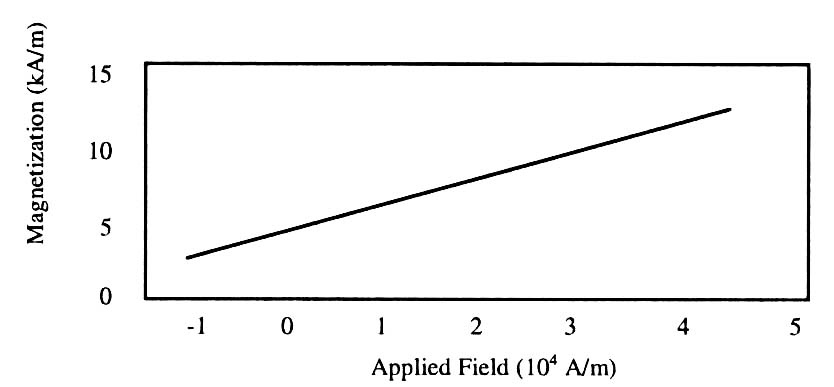
\includegraphics{figure1.jpg}
  \caption{Magnetization as a function of applied field. Note how the caption is centered in the column}
  % Note that label MUST come AFTER caption. Otherwise, you'll not get proper references for the figure
  \label{fig:figure1}
\end{figure}

\subsubsection{Figure Labels}

Use words rather than symbols or abbreviations when writing Figure axis labels to avoid confusing the reader. As an example, write the quantity “Magnetization”, or “Magnetization, M”, not just “M”. If including units in the label, present them within parentheses. Do not label axes only with units. In the example, write “Magnetization (A/m)” or “Magnetization {A[m(1)]}”, not just “A/m”. Do not label axes with a ratio of quantities and units. For example, write “Temperature (K)”, not “Temperature/K”.

\subsection{Footnotes}

Footnotes should be written using standard \LaTeX{} features\footnote{Like this footnote}.

\subsection{References}

The template will number citations consecutively within brackets \cite{eason1955certain}. The sentence punctuation follows the bracket \cite{maxwell1873treatise}. Refer simply to the reference number, as in \cite{jacobs1963fine} -- do not use “Ref. \cite{jacobs1963fine}” or “reference \cite{jacobs1963fine}” except at the beginning of a sentence: “Reference \cite{jacobs1963fine} was the first \ldots”

Unless there are six authors or more give all authors' names; do not use “et al.”.

Papers that have not been published, even if they have been submitted for publication, should be cited as “unpublished” \cite{elissa}. Papers that have been accepted for publication should be cited as “in press” \cite{nicole}. Capitalize only the first word in a paper title, except for proper nouns and element symbols.

For papers published in translation journals, please give the English citation first, followed by the original foreign-language citation \cite{yorozu1987electron}.

\section*{acknowledgment}

The preferred spelling of the word “acknowledgment” in America is without an “e” after the “g”. Avoid the stilted expression, “One of us (R. B. G.) thanks . . .”  Instead, try “R. B. G. thanks”. 

\bibliographystyle{IEEEtran}
\bibliography{references}

\end{document}
